\documentclass[a4paper,titlepage,11pt]{scrreprt}
\usepackage[top=3cm, bottom=2.5cm, left=2.5cm, right=2.5cm]{geometry}    
\usepackage[round]{natbib}
\usepackage{hyperref}
\usepackage{graphicx}
\usepackage{epstopdf}
\usepackage{helvet}
\usepackage[font=small,format=plain,labelfont=bf,up,textfont=normal,up, justification=justified,singlelinecheck=false]{caption}

\bibliographystyle{plainnat}

\renewcommand{\familydefault}{\sfdefault}


\parskip 12pt
\parindent 0pt
\renewcommand*{\chapterheadstartvskip}{\vspace*{-1.5cm}}


\linespread{1.5}

\begin{document}


\begin{titlepage}
\vspace*{1cm}
\begin{center}
\huge
\textbf{Tutorial for the speciesgeocodeR package}\\
\vspace{1cm}
\Large {Alexander Zizka  \today} \\
\end{center}

\vspace{1.5cm}
\Large

\normalsize

\textbf{Abstract}  SpecisgeocodeR is an R package designed for the analysis of species occurrences datasets linked with geographical polygons. It is a tool especially suited for bio-geographical and ecological questions, such as the distribution of specimens and species in geographic areas (e.g. biomes, or national park borders), particularly using large datasets. Based on a list of point coordinates (specimen occurrences) and a list of points building the polygons (geographical areas) speciesgeocodeR handles the classification of geographic points to geographical areas (point in polygon test) and runs multiple statistical analyses to summarize the results. An easy-to-use wraper function allows the run of a standard analysis with only 3 commands, making the package suited also for R beginners. The standard output includes a nexus file to use the results as direct input for bio-geographic analysis linked with phylogenetic trees, as well as summary tables, -graphs and geographical maps. Further functionalities include the direct use of the WWF ecoregions and biomes as input-polygons, calculating a co-occurrence matrix, producing diversity and abundance rasters from point occurrences and plotting diversity maps color-coding species diversity.

\end{titlepage}

\tableofcontents

\chapter{Introduction}

Ecological and bio-geographical research as well as conservation related studies often include questions on the spatial distribution of individuals and species. Point-occurrence information based on field collected GPS data, geo-referenced collection specimens or radio-collar reportings are nowadays one of the major sources for this data. For many analyses the relation of point-occurrences with geographical areas, such as continents, ecoregions, biomes or country and national park borders are of high interest. The large amount of point-occurrence data now available for many taxa (easily reaching tens of thousands up to millions of single data-points) together with the common use of multiple geographical areas for large-scale analysis renders the manual relation between occurrence points and areas a increasingly hopeless exercise.

SpeciesgeocodeR is an R package containing a set of functions to explore the relation of point (occurrence points) and polygon (geographic areas) data. This includes summarizing and preparing the data for further analyses. One main focus of the package is to provide an easy-to-use wrapper function to allow the use of a standard analysis for R beginners. A  standard standard analysis based on two input files in text format and the output includes a classification of each sample to each polygon in nexus and table format as well as a set of summary tables and graphs. Furthermore occurrence maps are created for every species and polygon of the input dataset. Further functionalities of the package include the calculation and visualization of a co-occurrence matrix, the direct use of the WWF terrestrial ecoregions as input areas, the creation of rasterized diversity and abundance maps as well as the production of maps color-coding species diversity per area.

The purpose of this tutorial is to provide easy-to-use instructions for the speciesgeocodeR package for R beginners, and to explain the functionality of the package to more advanced users. Chapter \ref{input}  specifies the input-file format, chapter \ref{allinone} provides a 3-step tutorial to run a standard analysis, chapter  \ref{wwf} describes how to use the WWF ecoregions as input polygons and chapter  \ref{output} describes the standard outputfiles. Chapter \ref{further} provides examples for the additional functions of the package. Chapter \ref{functions} contains a description of all functions in the package and chapter \ref{benchmark} shows results of benchmarking tests to give an idea of the computational time needed depending on the size of a dataset. Explanatory text is set in standard font, code examples are set in \texttt{teletypefont}.  All example scripts are also provided in a text-file with the package, so that the code can be copied directly from there into the R console. Although speciesgeocoder is explicitly designed for R-beginners some basic experience in using the R interface is surely helpful. If you have no experience with R you might want to have a look at \citet{crawley2012} or use the python version of Speciesgeocoder \citep{topel2014} instead. SpeciesgeocodeR is based on functions of the
maps \citep{becker2013}, maptools \citep{bivand2013b}, raster \citep{hijmans2014}, rgeos \citep{bivand2014} and sp \citep{pebesma2005, bivand2013}  packages.
\chapter{Input files} \label{input}

Most analyses possible with speciesgeocodeR are based on two input files. These can easily be generated using freely available text-formatting and GIS software: a list of sample coordinates (e.g. GPS-coordinates of specimen, hereafter called ``speciesdata") and a list of polygon points (e.g biomes or national park borders, hereafter called ``polygondata"). The package is designed and tested for small-scale (e.g. radio-colar data in combination with national park borders) and large scale (e.g global distribution of all birds to biomes) analyses. If you want to use the WWF classification, or create a diversity grid, no separate input polygon file is needed. (see chapters \ref{wwf} and \ref{further})

\textit{Input}-files: The two input files are required to be tab-delimited .txt files with three columns each. For both files, column names must be: �identifier�, �XCOOR�, YCOOR�. In case of the speciesdata the first column contains the species name (or individual name), the second column contains the longitude coordinates (as decimal degrees, e.g. 59.867 for East, or -59.867 for West) and the third column contains latitude coordinates (as decimal degrees, e.g. 59.867 for North, or -59.867 for South). The polygondata should be in the same format: each row represents the coordinates of one polygon corner. The first column contains the polygon identifier, the second one the longitude coordinates, the third one the latitude coordinates. It is important that the coordinates of the first and the last point of each polygon are identical. Example input files are provided with the package (in the example\_files folder). You can easily export such a file from any GIS program (e.g. QGIS \citealt{qgis}). If you use  polygondata exported from QGIS or formated for the python version of speciesgeocoder you can use the ConvertPoly() function to convert the format.

When preparing the input files please make sure:
\begin{enumerate}
\item that the order of the columns and the column headers are correct (``identifier", ``XCOOR", ``YCOOR")
\item that your coordinates conform with the limits of the coordinate system (XCOOR between -180 and 180; YCOOR between -90 and 90)
\item that for each polygon in the polygondata the first and last point have identical coordinates.
\end{enumerate}

\chapter{SpeciesGeoCoder all-in-one: the quick and easy way} \label{allinone}

You can run a standard speciesgeocoder analysis with only three commands. The example code shown here is also provided as text file with the package so if you are unfamiliar with the R environment, you can just copy the example code from there to the R console (the capitalized phrases correspond to your filenames and must be changed accordingly). We will use a distribution dataset from the Rosaceae genus \textit{Ivesia} in western North America from Mats T\"opel \citep{topel2012} as example dataset. If you are interested in a step by step process or in the use of single functions refer to chapters five and six:

\begin{enumerate}

\item  Create a new folder in your home directory (the working directory). At the moment speciesgeocodeR is provided as .zip file. Copy the speciesgeocodeR.zip into your working directory and extract it there. The copy your two input files into the working directory and give them characteristic names (here we will use ``ivesia\_coordinates.txt'' for our speciesdata and ``ivesia\_polygons.txt'' for the polygondata, from the example\_data subfolder). If you are insecure about the format of your input files or an error occurs right away, check chapter one of this manual or take look at the example files delivered with the package.

\item Start R

\item Tell R where to find the input files and save the outputfiles. You must put the exact path of your working directory in the quotation marks (e.g. ``C:\textbackslash \textbackslash Desktop\textbackslash \textbackslash data''). If you use mac (or linux) use / instead of \textbackslash \textbackslash.

\texttt{setwd(``YOUR WORKING DIRECTORY PATH'')}

\item Load the functions of the speciesgeocoder package into your R session 

\texttt{source(``speciesgeocodeR.R'')}

\item{Execute the SpeciesGeoCoder() function with the names of your two input files as arguments (e.g ``ivesia\_coordinates.txt'', ``ivesia\_polygons.txt''). Depending on the size of your dataset this might take a while. The �graphs� argument controls if graphical output is produced (default = T), the``coex"' argument defines if a coexistence matrix for all species in each polygon is produced (default = F, this is only recommended for datasets with small to medium size species number, as it is computationally very intense)}

\texttt{SpeciesGeoCoder(``example\_data\textbackslash \textbackslash ivesia\_coordinates'', }\\
\texttt{``example\_data\textbackslash \textbackslash ivesia\_polygons'',  graphs = T, coex = F)}

\item{Done! Close R, the output files are in your working directory. Summary tables are saved as tab-delimited .txt files, graphs and maps as .pdf files. If problems occur, check your input-files or try using one of the example datasets delivered with the package. If this does not help, you might want to use the step-by-step procedure described in chapter \ref{further}.}

\item{If your polygondata input file is exported from QGIS and/or is formated for use with the python version of speciesgeocodeR, you can use the ConvertPoly() function to convert it to a format suitable for use with speciegeocodeR.}

\texttt{setwd(``YOUR WORKING DIRECTORY PATH'')}\\
\texttt{source(``speciesgeocodeR.R'')}\\
\texttt{poly \textless- ConvertPoly(``example\_data\textbackslash \textbackslash ivesia\_polygons\_python\_format.txt'')}\\
\texttt{write.table(poly, ``example\_data\textbackslash \textbackslash ivesia\_polygons\_reformat.txt'', row.names = F,  sep = ``\textbackslash t'')}\\
\texttt{SpeciesGeoCoder(``example\_data\textbackslash \textbackslash  ivesia\_coordinates'', }\\
\texttt{``example\_data\textbackslash \textbackslash ivesia\_polygons\_reformat.txt'',  graphs = T, coex = F)}
\end{enumerate}

\chapter{Using the WWF Realms/Biomes/Ecoregions as input polygons} \label{wwf}

The map of the terrestrial ecoregions of the world as provided by the WWF \citep{olson2001}, is a helpful tool for bio-geographical analyses. If you want to classify the samples in your dataset using these ecoregions/biomes/realms, you can directly use them as input-polygons for speciesgeocodeR. To do so, just use the WWFload() function which will download the a shape file from the WWF homepage.  You can use the object created by this function directly as input-polygon for SpeciesGeoCoder(). When you run SpeciesGeoCodeR() with WWF input polygons you must specify two additional arguments: ``wwf = T'' and scale = ``ECOREGION'' (or ``BIOME'' or ``REALM''). This defines the scale at which the results will be displayed in the output. If as in the example scale = ``BIOME'' the species numbers will be summarized per biome: 

\texttt{setwd(``YOUR WORKING DIRECTORY PATH'')}\\
\texttt{source(``speciesgeocodeR.R'')}\\
\texttt{wwf \textless- WWFload()}\\
\texttt{SpeciesGeoCoder(``example\_data\textbackslash \textbackslash  ivesia\_coordinates'', wwf,  graphs = T, coex = F, wwf = T, scale = "BIOME")}

If you want to use a subset of the global WWF dataset, you can use WWFnam() to display all possible ecoregions, biomes and realms. Subsequently you can use WWFpick()  to create a subset of the global dataset. The WWFpick() function needs three  arguments: x = the object where the global wwf shape is stored (wwf in the example); scale  = the scale of the region you want to pick. This must be one of the following: ``ECOREGION'', ``BIOME'' or ``REALM' '(but does not need to be the same as the scale argument used later in the SpeciesGeoCoder() function);  name = the name(s) of the ecoregion, biome or realm you want to pick, e.g. ``Nearctic''. This can also be a vector of multiple elements of one scale e.g. c(``Nearctic'', ``Neotropics''), but must correspond to the scale indicated by the scales argument. You can use the WWFnam() function for an overview of available regions on each scale.

\texttt{WWFnam(wwf)}\\
\texttt{poly \textless- WWFpick(wwf,  scale = ``REALM'', name  = ``Nearctic'')}\\
\texttt{SpeciesGeoCoder(``example\_data\textbackslash \textbackslash  ivesia\_coordinates'', poly,  graphs = T, coex = F, wwf = T, scale = " BIOME") }

If you have trouble with the WWFload() function you can also download and unzip the files manually  (e.g. from \citealt{wwfeco}\\
 and copy them in your working directory. Then you can load them into R as following

\texttt{setwd(``YOUR WOKINGDIRECTORY PATH'')}\\
\texttt{source(``speciesgeocodeR.R'')}\\
\texttt{wwf \textless- readShapeSpatial( ``wwf\_terr\_ecos.shp'')}

\chapter{Output-file description} \label{output}

With the ``graphs'' and ``coex'' options swiched on, SpeciesGeoCoder() produces 13 output files by default (1 nexus file, 5 summary tables, 3 barcharts, 3 maps and 1 heatplot). All files are saved to the working directory defined before the analysis. The summary tables are tab delimited .txt files and all graphics and maps are saved as .pdf files. Depending on the size of you dataset, some of the graphical representations might not be adequate. \\
\\
\textbf{Barchart\_per\_polygon.pdf}\\
This file contains one barchart for each input polygon showing the total number of occurrences for each species in this polygon.\\
\textbf{Barchart\_per\_species.pdf}\\
This file contains one barchart per species, showing the relative number of occurrences in each input polygon.\\
\textbf{Heatplot\_coexistence.pdf}\\
This file contains a heat plot showing the co-existence pattern of all species in the analysis. This output is turned of by default. To turn it on, use  ``coex = T'' as argument of the SpeciesGeoCoder() function.\\
\textbf{Map\_samples\_overview.pdf}\\
This file contains  an overview map showing all input points and polygons.\\
\textbf{Map\_samples\_per\_polygon.pdf}\\
This file contains one map for each input polygon, showing all occurrence points included in the polygon color-coded for species.\\
\textbf{Map\_samples\_per\_species.pdf}\\
This file contains one map  for each input species showing all polygons and all occurrence points of this species. Point samples classified to any polygon are shown in blue, unclassified samples are shown in red.\\
\textbf{Numer\_of\_species\_per\_polygon.pdf}\\
This file contains a barchart indicating the number of species per polygon.\\
\textbf{Species\_classification.nex}\\
This is a nexus file containing the area coding for each species (1 = occurrence, 0 = absence) for biogeographic analysis in combination with phylogenetic data.\\
\textbf{Sample\_classification\_to\_polygon.txt}\\
This is a summary table showing the classification for each sample point.\\
\textbf{Species\_occurrence\_per\_polygon.txt}\\
This is a summary table showing the presence or absence of every species in the input polygons.\\
\textbf{Species\_number\_per\_polygon.txt}\\
This is a table summarizing the number of species for each polygon.\\
\textbf{Unclassified\_samples.txt}\\
This file contains a map showing all samples that could not be classified to any of the input polygons.\\

\chapter{Further functionalities} \label{further}
\section{Calculating a co-existence matrix} \label{coex}
Understanding coexistence patterns is a crucial aspect of ecology and biogeography. Based on the two input files used in the previous chapters (or one inputfile and the WWF ecoregions)you can calculate a coexistence matrix and it visualize it as a levelplot. This can be done in two different ways:

\begin{enumerate}
\item{When running a normal analysis, by setting coex = T in the SpeciesGeoCoder() function. In this case the matrix is saved as .txt file in the working directory and the levelplot (only for datasets \textless 40 species) is saved as .pdf in the working directory.  However, this is only recommended for small datasets, as the computation might take a long time. This can also be combined with the use of the WWF ecoregions as shown in chapter 3.}

\texttt{setwd(``YOUR WORKING DIRECTORY PATH'')}\\
\texttt{source(``speciesgeocodeR.R'')}\\
\texttt{SpeciesGeoCoder(``example\_data\textbackslash \textbackslash ivesia\_coordinates.txt'',}\\
\texttt{ ``example\_data\textbackslash \textbackslash ivesia\_polygons.txt'',  graphs = T, coex = T)}

\item{More efficiently, the coexistence matrix calculation can can also be calculated without the wrapper function. To do this you must first load the input data using the ReadPoints() function and run the SpGeoCodH() function which creates an object of the class ``spgeoOUT'' (it runs speciesgeocoder without output files). This object can be used with the CoExClass() function to create the coexistence matrix.}

\texttt{inp\_ivesia  \textless- ReadPoints(``example\_data\textbackslash \textbackslash ivesia\_coordinates.txt'',}\\
\texttt{ ``example\_data\textbackslash \textbackslash ivesia\_polygons.txt'')}\\
\texttt{outp\_ivesia \textless- SpGeoCodH(inp\_ivesia)}\\
\texttt{coex\_ivesia \textless- CoExClass(outp\_ivesia)}

\item{For small datasets the matrix can then be plotted as a levelplot using HeatPlotCoEx().}
\texttt{HeatPlotCoEx(coex\_ivesia)}

\begin{center}
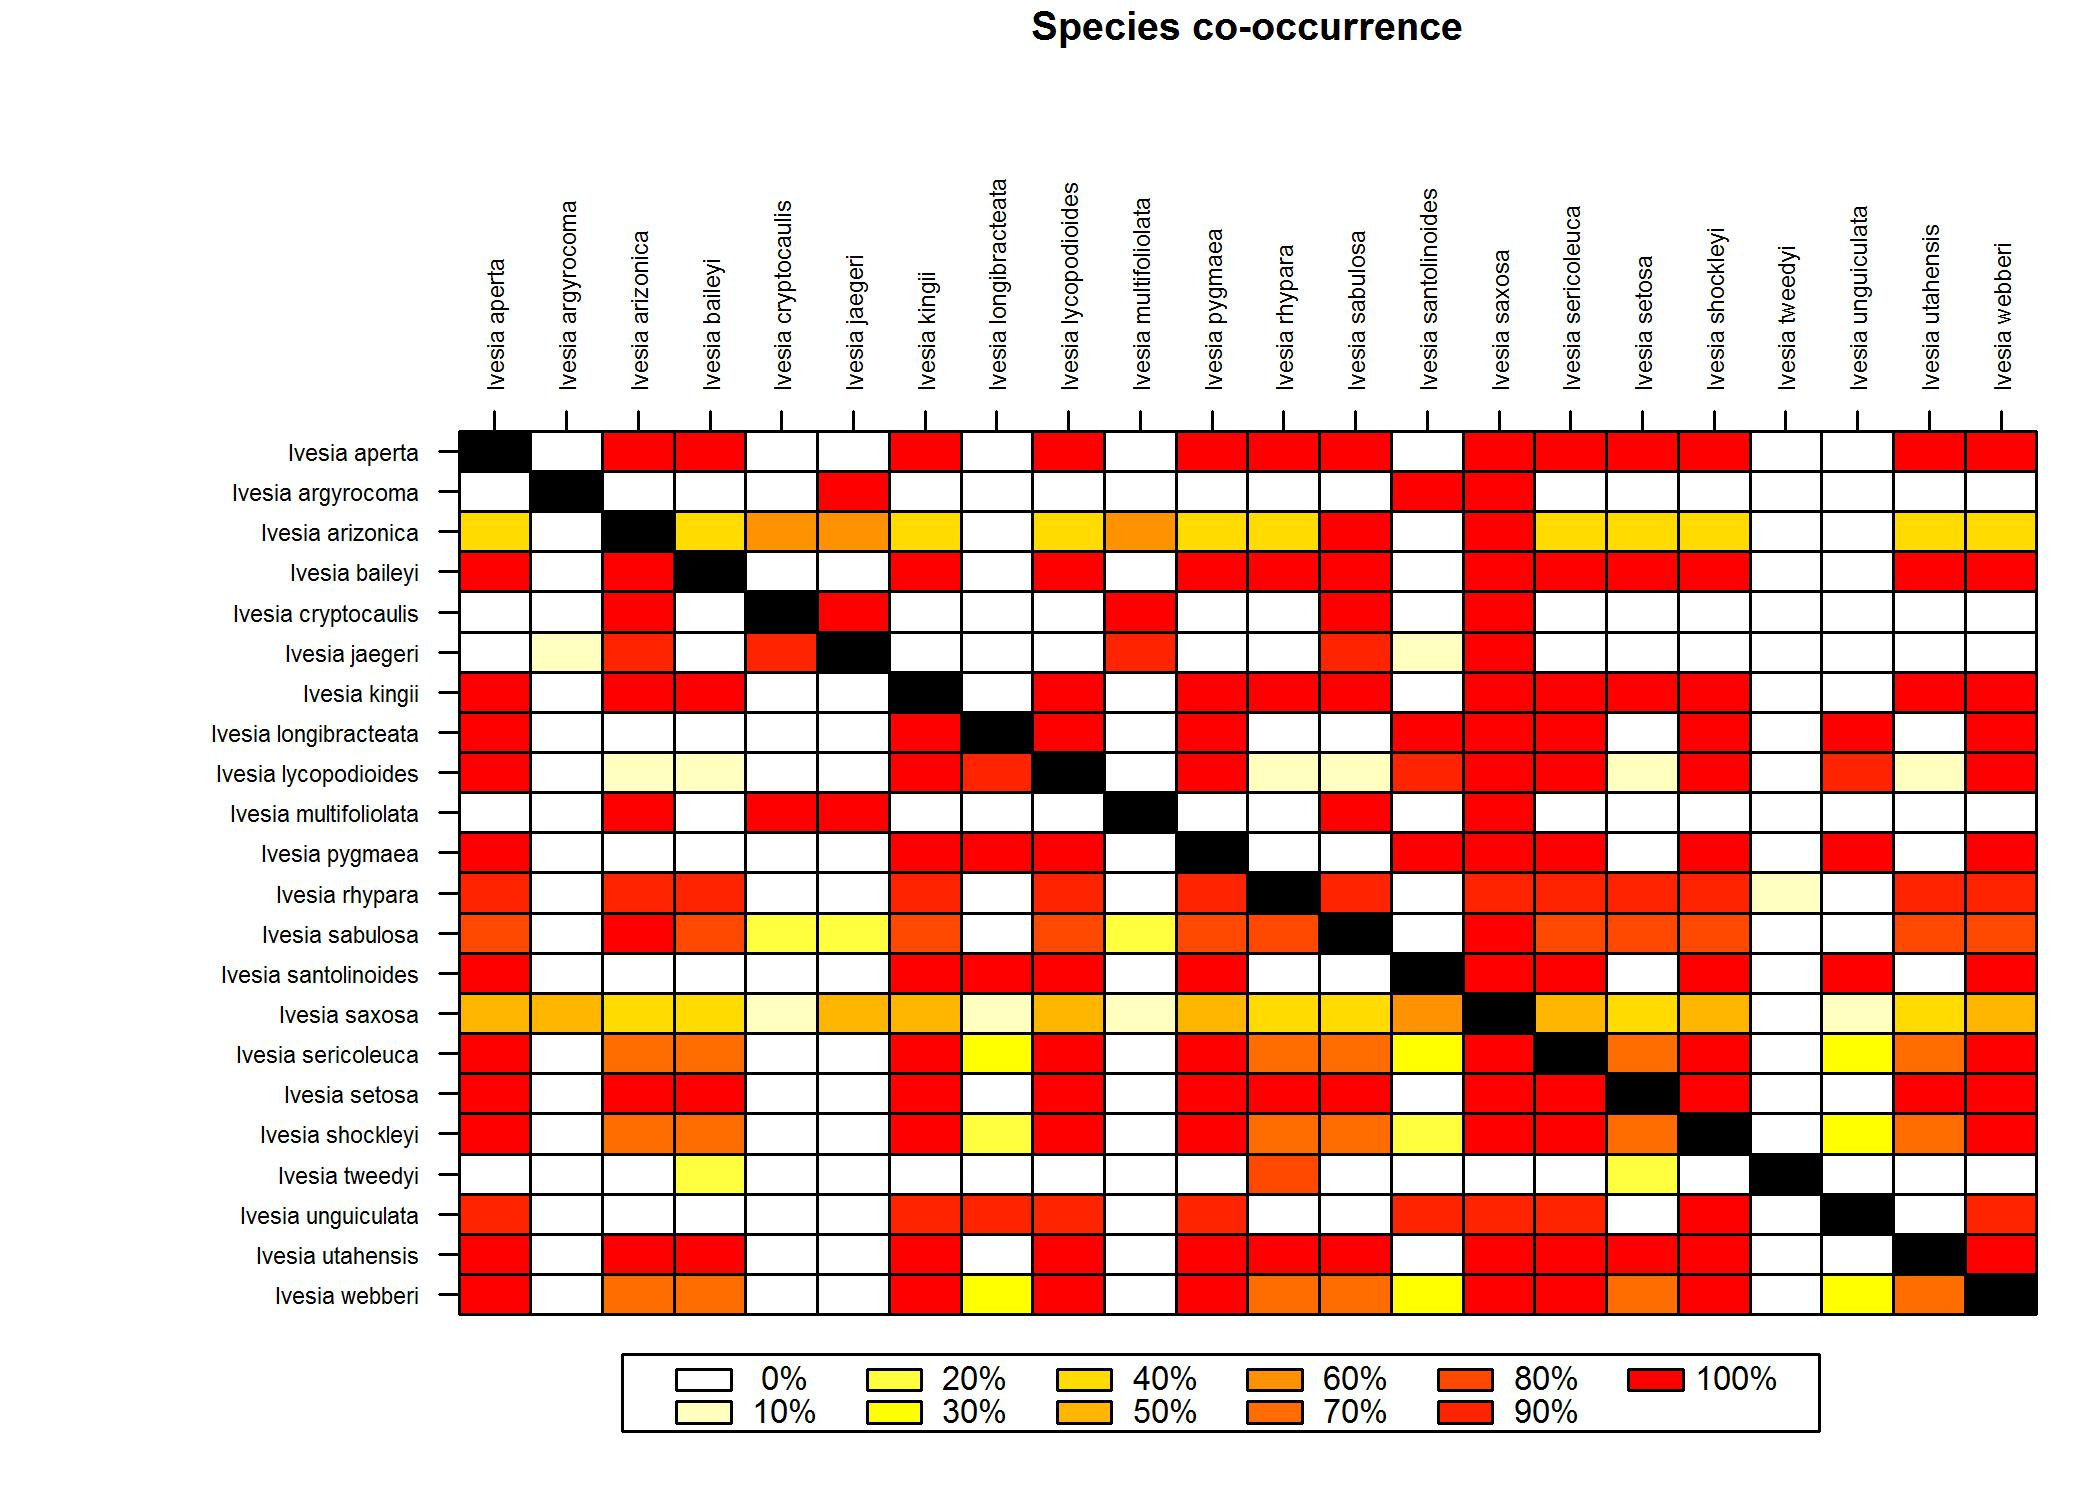
\includegraphics[width=0.9\textwidth]{figures/levelplot_ivesia.jpeg}
\end{center}

\item{If you want to use the WWF classification on biome or realm level you must include an additional step using the clust() function.}

\texttt{wwf \textless- WWFload()}\\
\texttt{poly \textless- WWFpick(wwf, scale = ``REALM'', name  = ``Nearctic'')}\\
\texttt{inp\_ivesia  \textless- ReadPoints(``example\_data\textbackslash \textbackslash ivesia\_coordinates.txt'', poly)}\\
\texttt{outp\_ivesia \textless- SpGeoCodH(inp\_ivesia)}\\
\texttt{clust\_ivesia \textless- clust(outp\_ivesia, poly, scale = ``BIOME'')}\\
\texttt{coex\_ivesia \textless- CoExClass(clust\_ivesia)}\\
\texttt{HeatPlotCoEx(coex\_ivesia)}

\end{enumerate}

\section{Mapping diversity in polygons}
Visualizing the species diversity in all areas of interest can be helpful to understand large scale patterns. The MapDiversity() function of speciesgeocodeR can be used to color-code diversity in the input polygons. 

If you want to use polygons imported from a text file, you must first load the data and run SpeciesGeoCoder() as in \ref{coex}. Then you can use the MapDiversity() function on the output object. When using the MapDiversity() function with data imported from text files you must specify scale = ``CUSTOM''.

\texttt{inp\_ivesia  \textless- ReadPoints(``example\_data\textbackslash \textbackslash ivesia\_coordinates.txt'', }\\
\texttt{``example\_data\textbackslash \textbackslash ivesia\_polygons.txt'')}\\
\texttt{outp\_ivesia \textless- SpGeoCodH(inp\_ivesia)}\\
\texttt{MapDiversity(outp\_ivesia, scale = "CUSTOM")}

\begin{center}
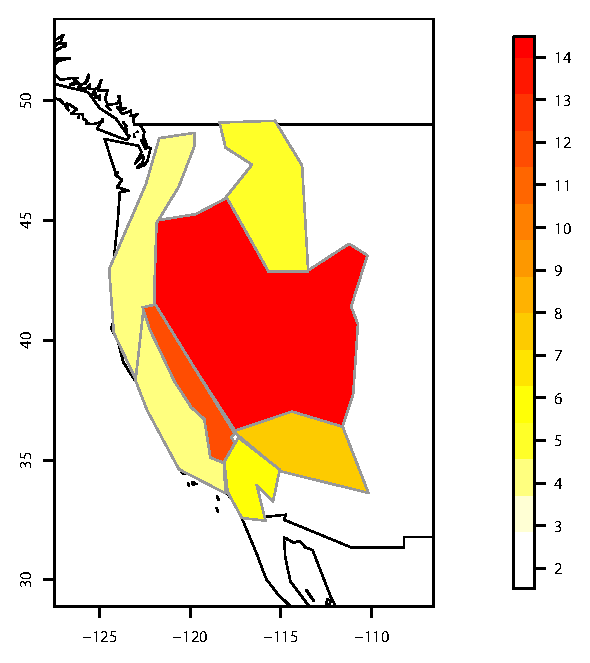
\includegraphics[width=0.55\textwidth]{figures/mapdiversity_continous.eps}
\end{center}

The MapDiversity() function has a number of additional arguments to control the appearance of the plot: leg = "continuous" or "discrete" defines the use of a continuous or discrete color scheme. When using neighboring areas with little difference in species number a the discrete coloring might be more helpful.

\texttt{MapDiversity(outp\_ivesia, scale = "CUSTOM", leg = ``discrete'')}\\
\begin{center}
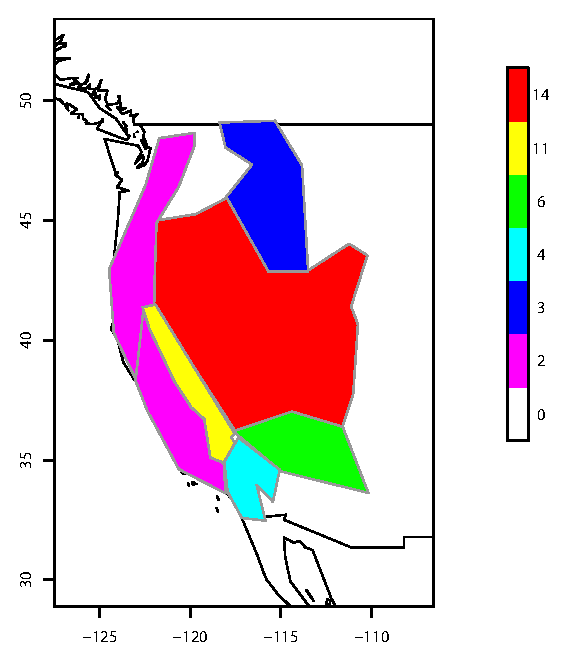
\includegraphics[width=0.55\textwidth]{figures/mapdiversity_discrete.eps}\\
\end{center}

The show.occ = T shows the occurrence points on the map (only with input from a spgeoOUT object).

\texttt{MapDiversity(outp\_ivesia, scale = "CUSTOM", leg = "continuous", show.occ = T)}\\
\begin{center}
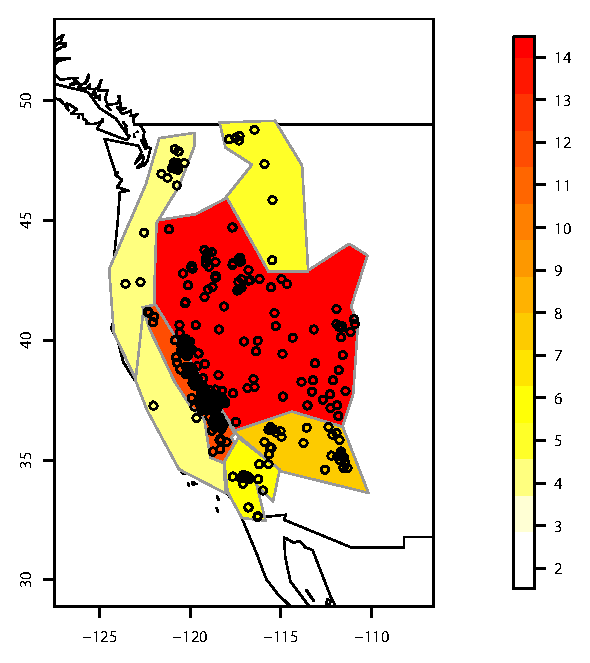
\includegraphics[width=0.55\textwidth]{figures/mapdiversity_points.eps}\\
\end{center}

You can also use the MapDiversity() function with polygons derived from the WWF ecoregions. Note that the scale argument must be changed accordingly. 

\texttt{wwf \textless- WWFload()}\\
\texttt{poly \textless- WWFpick(wwf, scale = ``REALM'', name  = ``Nearctic'')}\\
\texttt{inp\_ivesia  \textless- ReadPoints(``example\_data\textbackslash \textbackslash ivesia\_coordinates.txt'', poly)}\\
\texttt{outp\_ivesia \textless- SpGeoCodH(inp\_ivesia)}\\
\texttt{MapDiversity(outp\_ivesia, scale = "ECOREGION", leg = ``continous'')}\\

\begin{center}
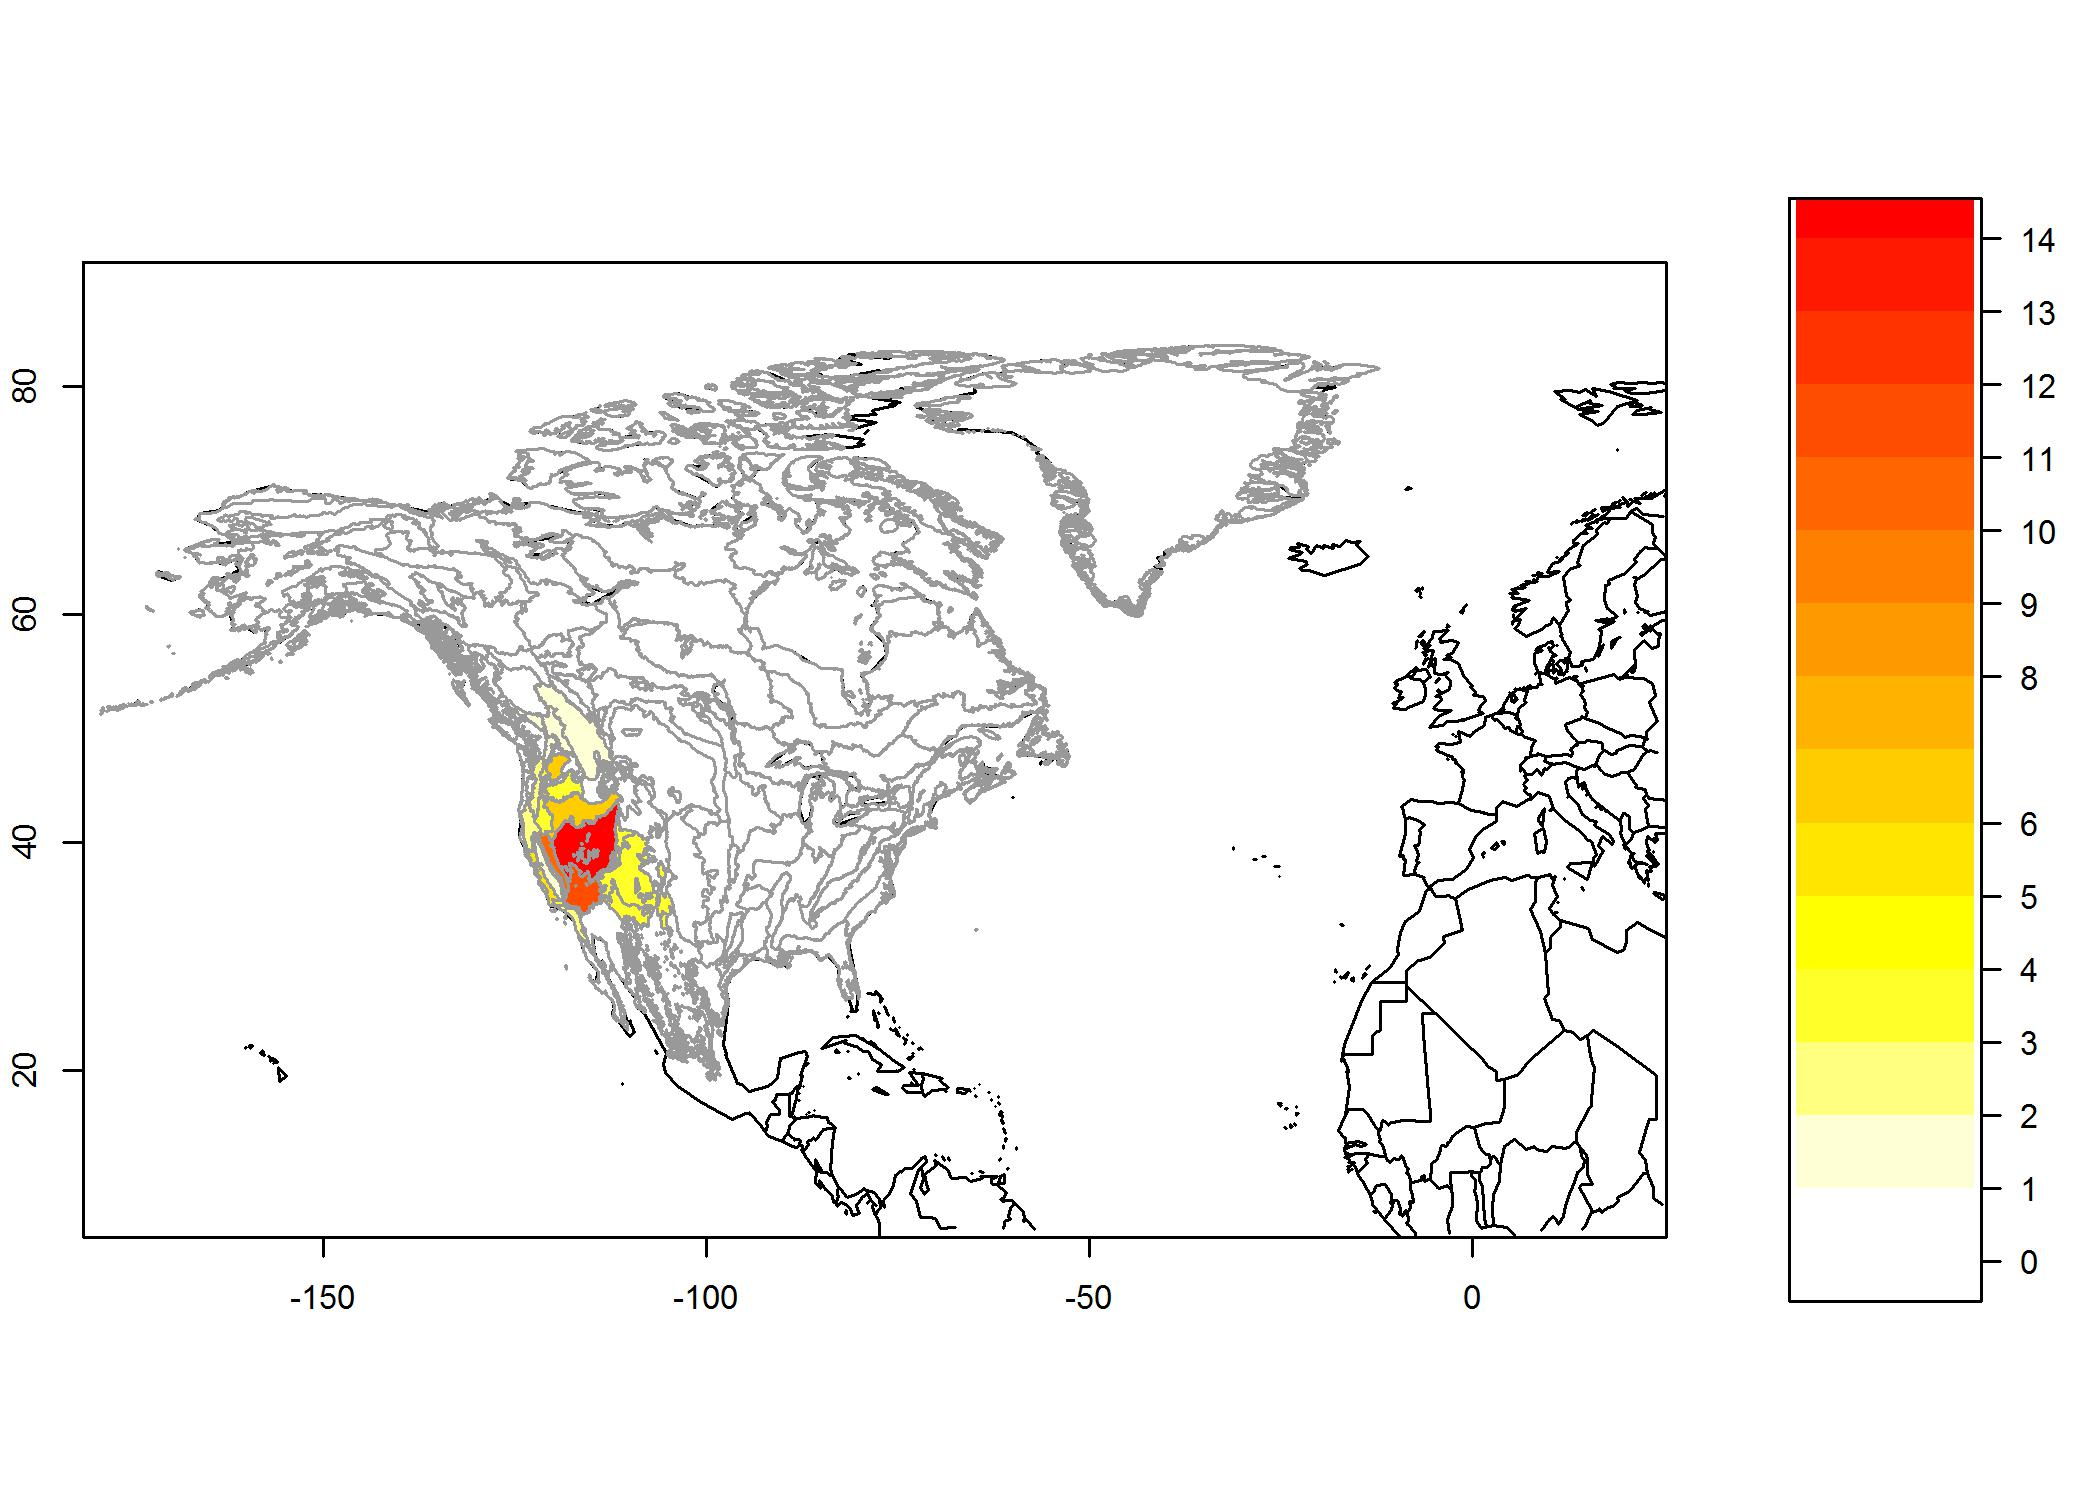
\includegraphics[width=0.7\textwidth]{figures/mapdiversity_ecoregions_polygons.jpeg}\\
\end{center}

In this cases where the polygons used cover a much larger area than the actual area of interest (as in this example where they stretch over entire North America), the lim argument can be used to adjust the pane shown on the map. lim = "polygons" or "points" defines if the points or polygons are used to define the plot outline.
\texttt{MapDiversity(outp\_ivesia, scale = "ECOREGION", leg = ``continuous'', lim = "points")}\\

\begin{center}
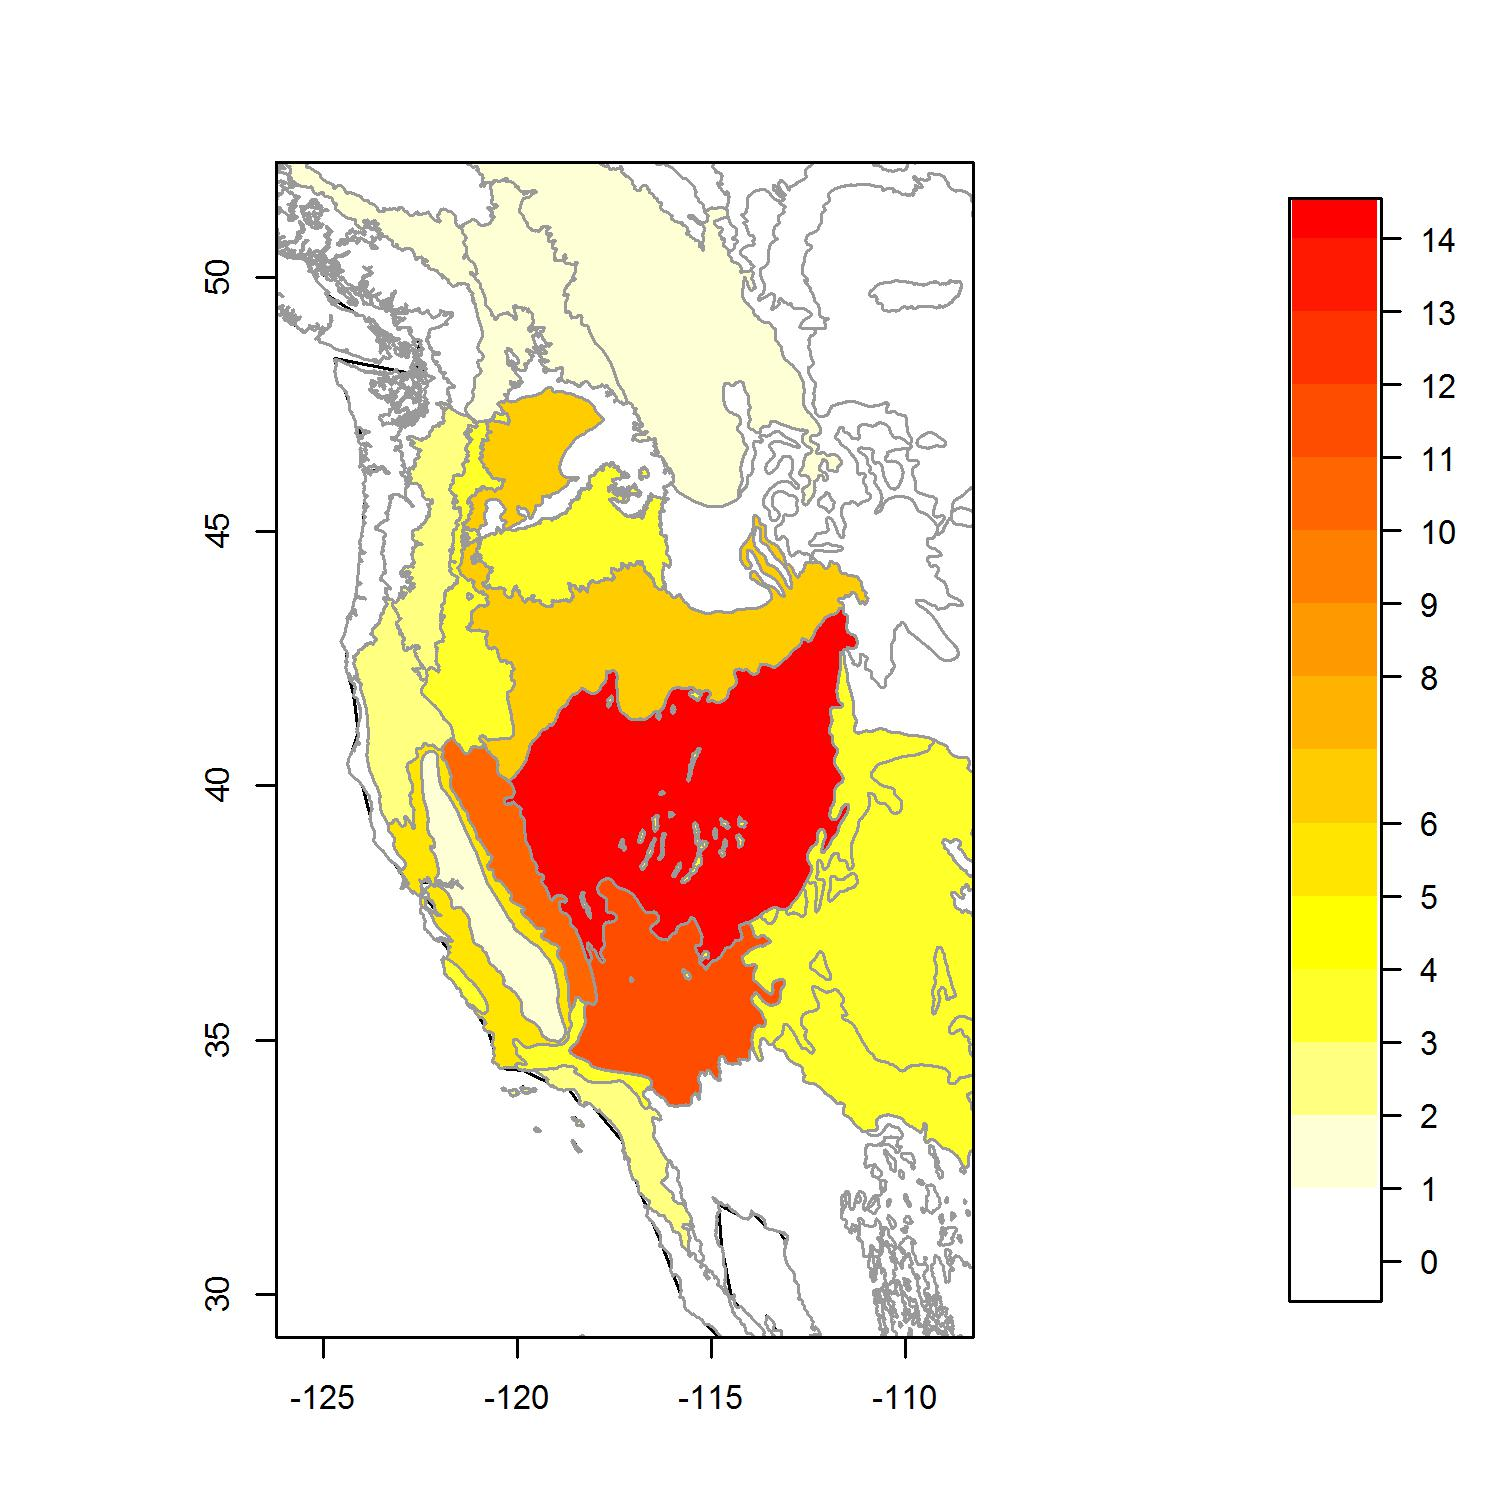
\includegraphics[width=0.55\textwidth]{figures/mapdiversity_ecoregions_points.jpg}\\
\end{center}

If you want to use the WWF  biomes or realms with the MapDiversity() function, the data must first be prepared using the clust() function. When using the WWF polygons as input you must also set the scale argument of the MapDiversity() function accordingly to either "BIOME" or "REALM". 

\texttt{wwf \textless- WWFload()}\\
\texttt{poly \textless- WWFpick(wwf, scale = ``REALM'', name  = ``Nearctic'')}\\
\texttt{inp\_ivesia  \textless- ReadPoints(``example\_data\textbackslash \textbackslash ivesia\_coordinates.txt'', poly)}\\
\texttt{outp\_ivesia \textless- SpGeoCodH(inp\_ivesia)}\\
\texttt{clust\_ivesia \textless- clust(outp\_ivesia, poly, scale = ``BIOME'')}\\
\texttt{MapDiversity(clust\_ivesia, scale = "BIOME", leg = ``continuous'')}\\

\begin{center}
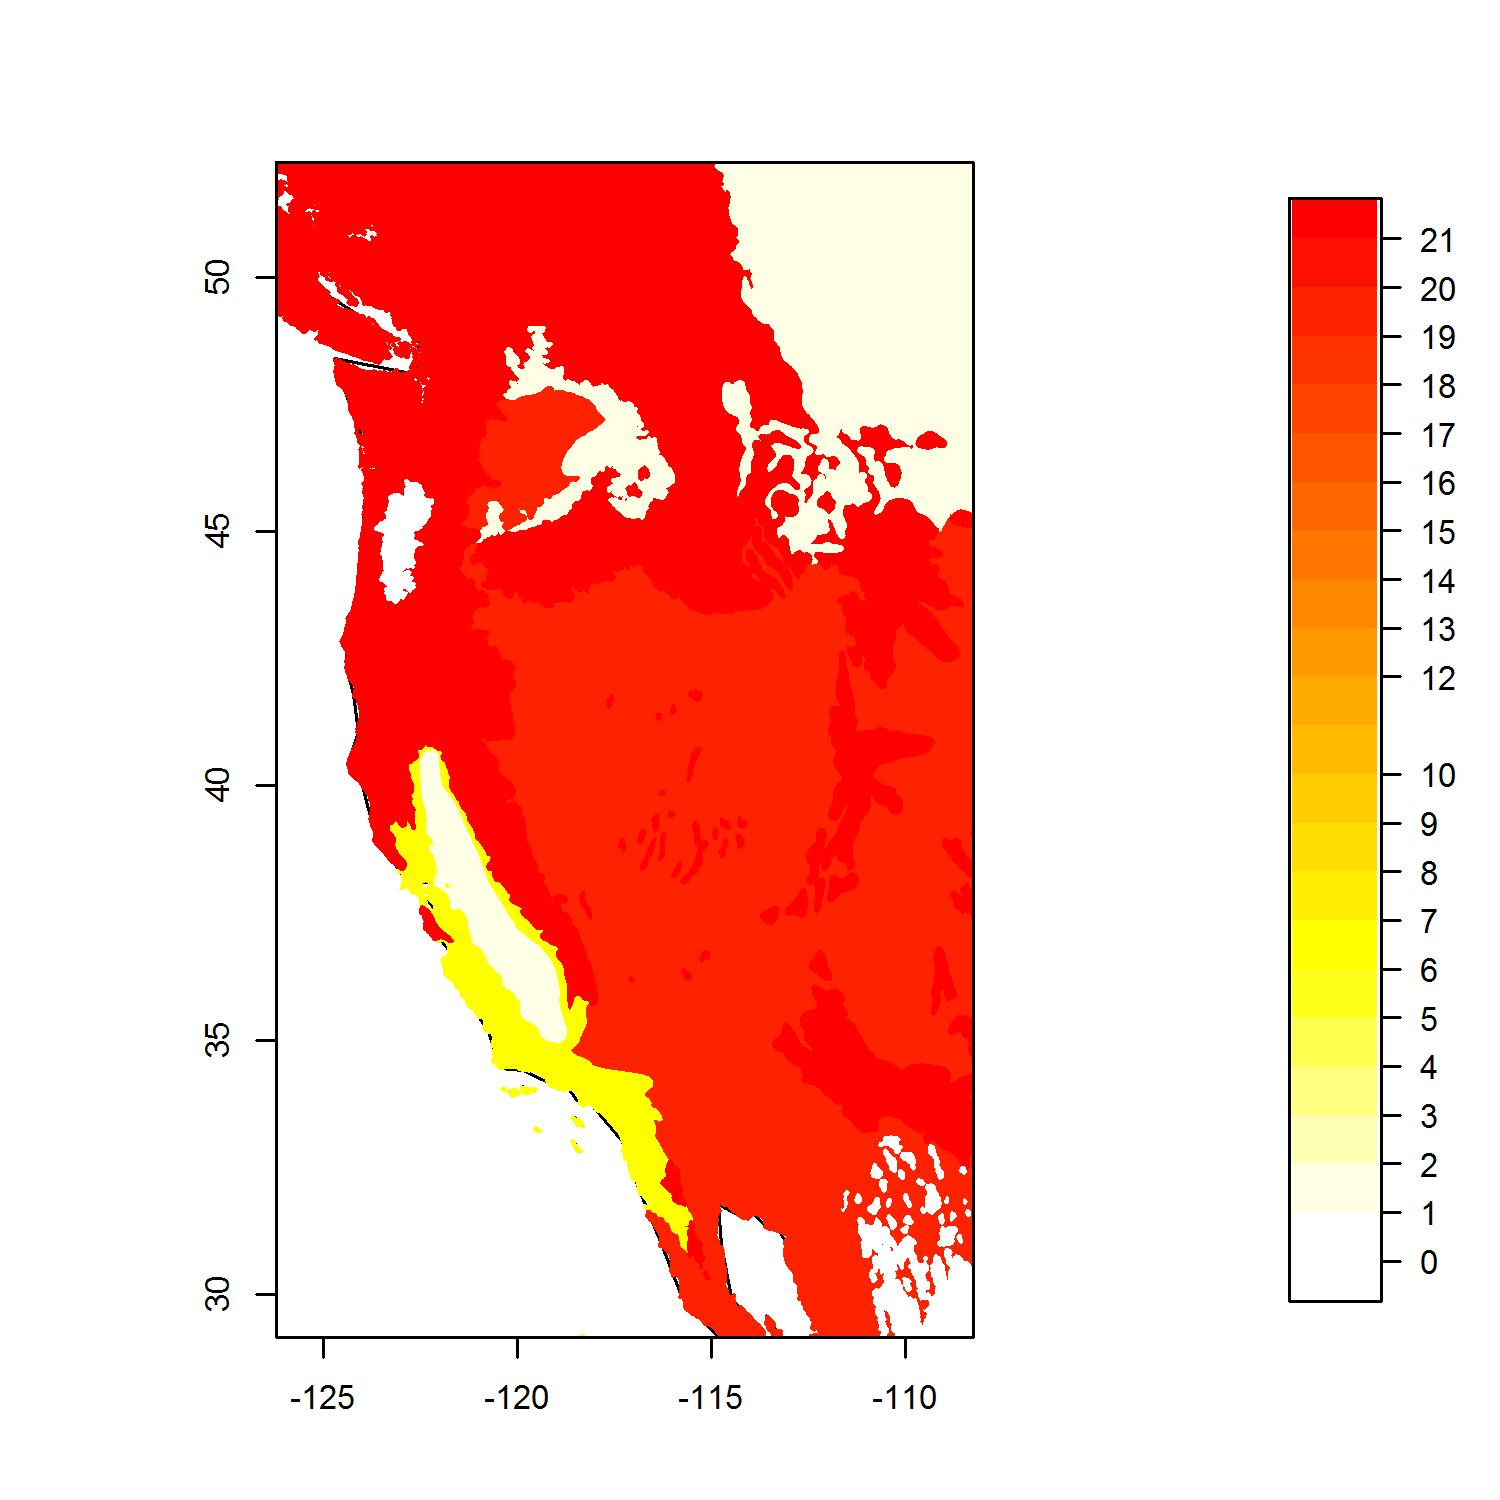
\includegraphics[width=0.7\textwidth]{figures/mapdiversity_biomes.jpg}\\
\end{center}

\texttt{clust\_ivesia \textless- clust(outp\_ivesia, poly, scale = ``REALM'')}\\
\texttt{MapDiversity(clust\_ivesia, scale = "REALM", leg = ``discrete'')}\\

\begin{center}
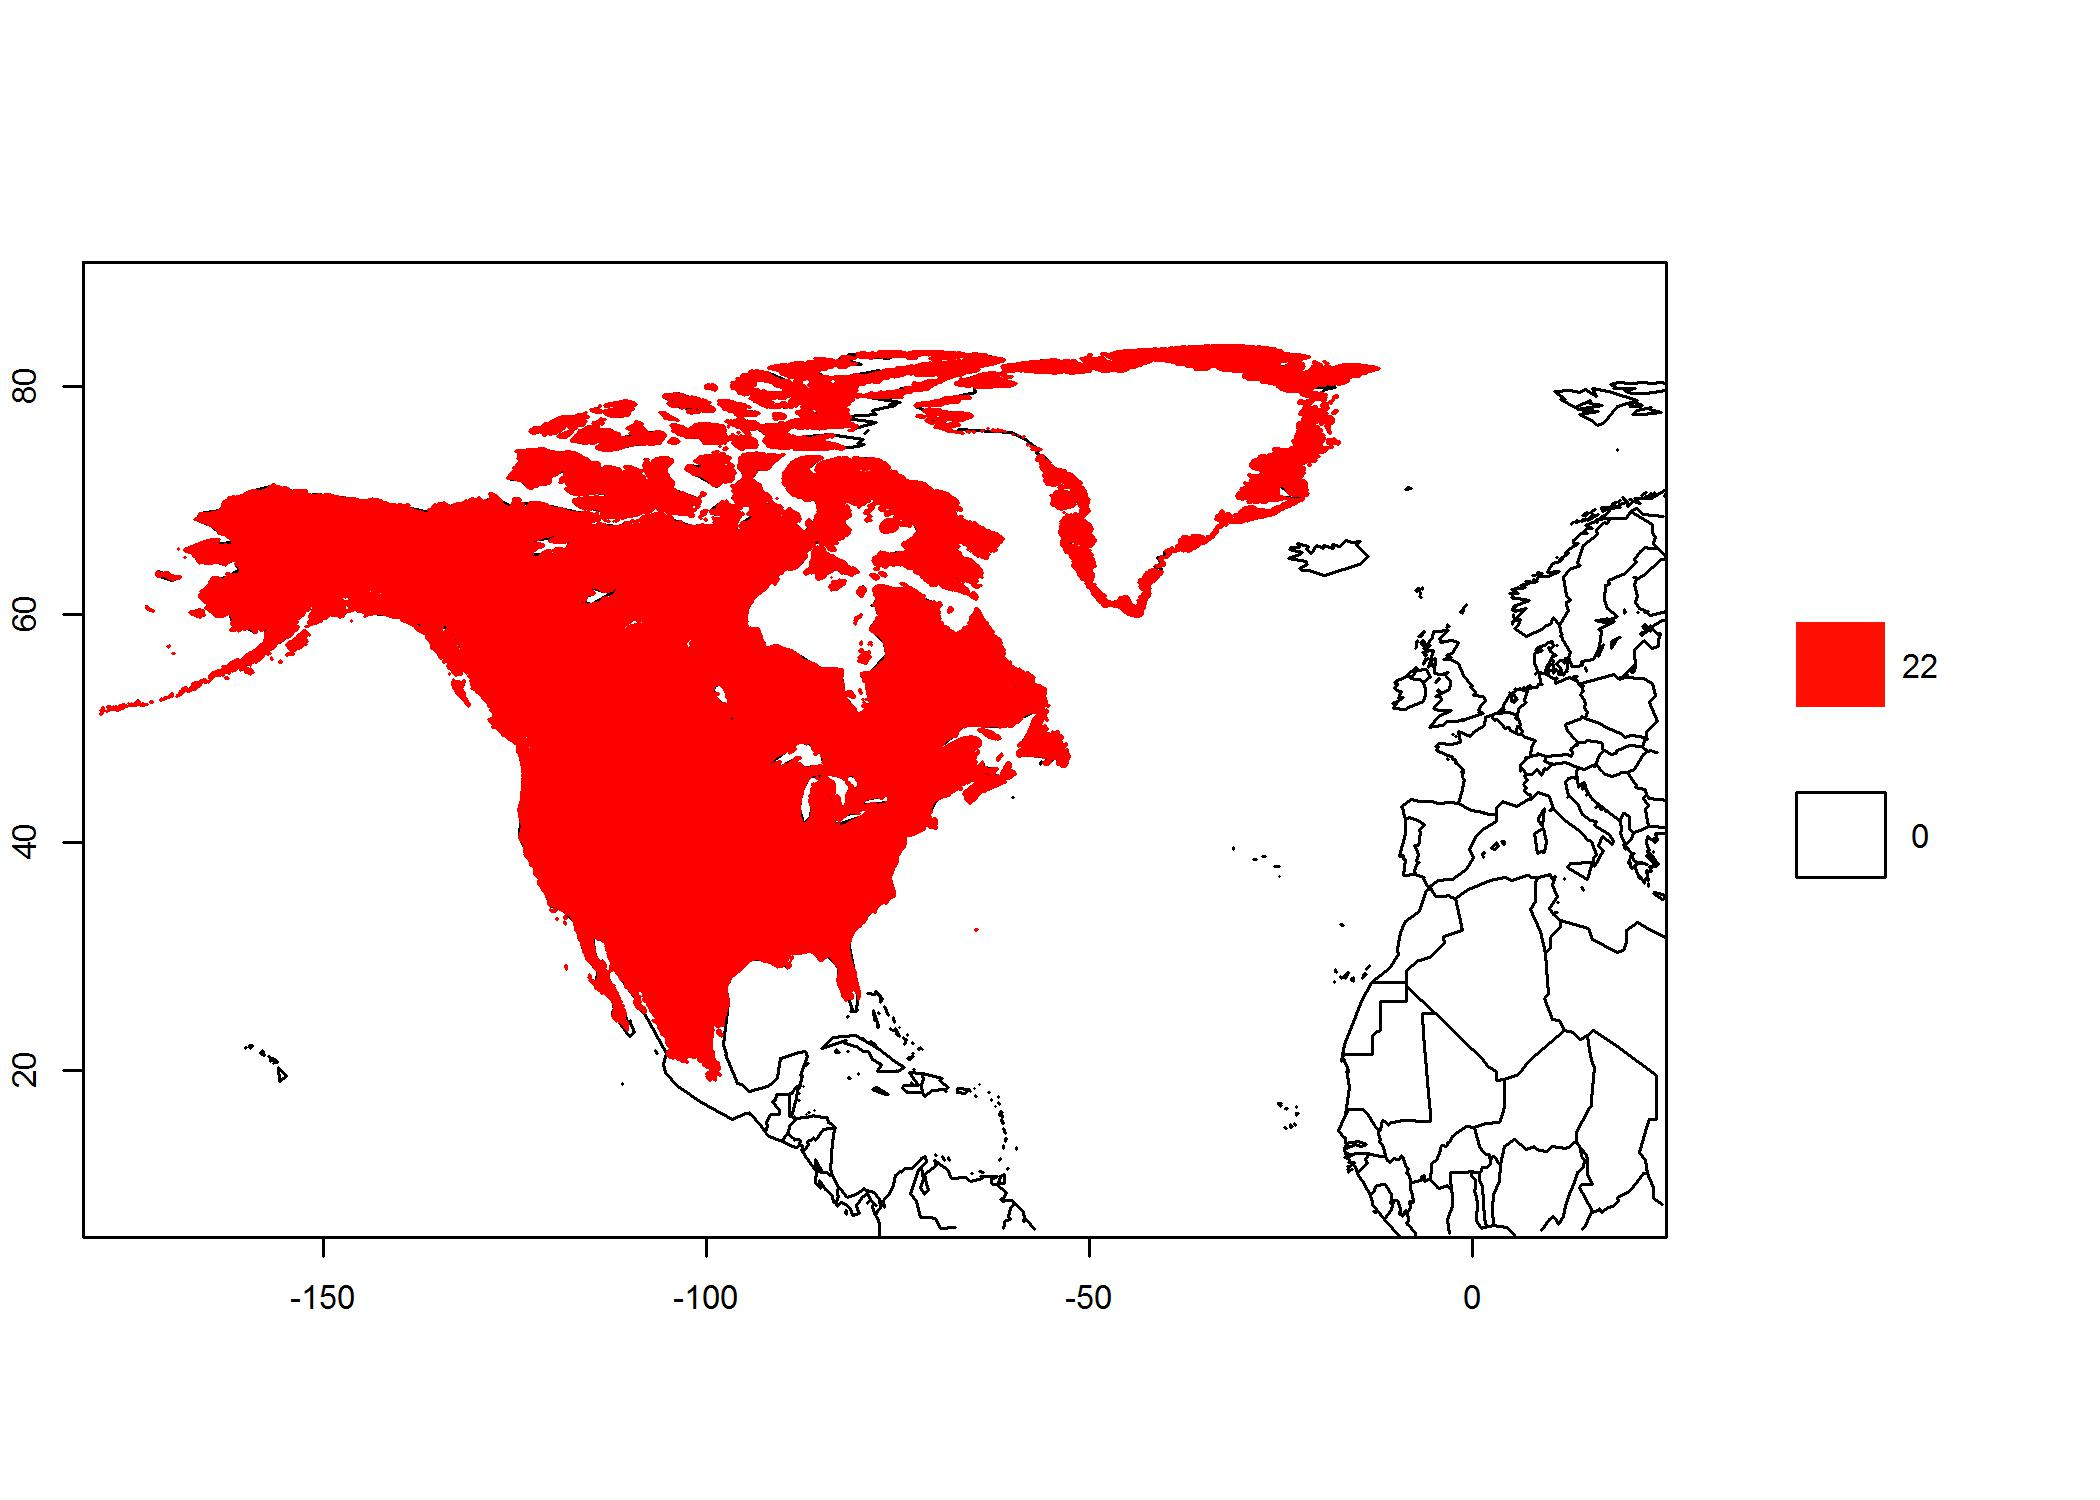
\includegraphics[width=0.7\textwidth]{figures/mapdiversity_realms.jpg}\\
\end{center}

\section{Diversity and abundance grids}
In some situations the visualization of diversity patterns in a raster is of interest. You can use the DiversityGrid() function to produce a one degree diversity raster of you data indicating the number of species per raster cell. The xlim and ylim arguments control the minimum and maximum coordinates for the raster:

\texttt{ivesia\_div \textless- DiversityGrid(``example\_data\textbackslash \textbackslash ivesia\_coordinates.txt'',xlim = c(-130,-105), ylim = c(30,50))}

This produces an object of the class raster, which can be handled with all the functions of the raster-package \citep{hijmans2014}. As an easy solution to plot the raster in the context of national borders you can use the MapGrid() function of speciesgeocodeR:

\texttt{MapGrid(ivesia\_div)}

\begin{center}
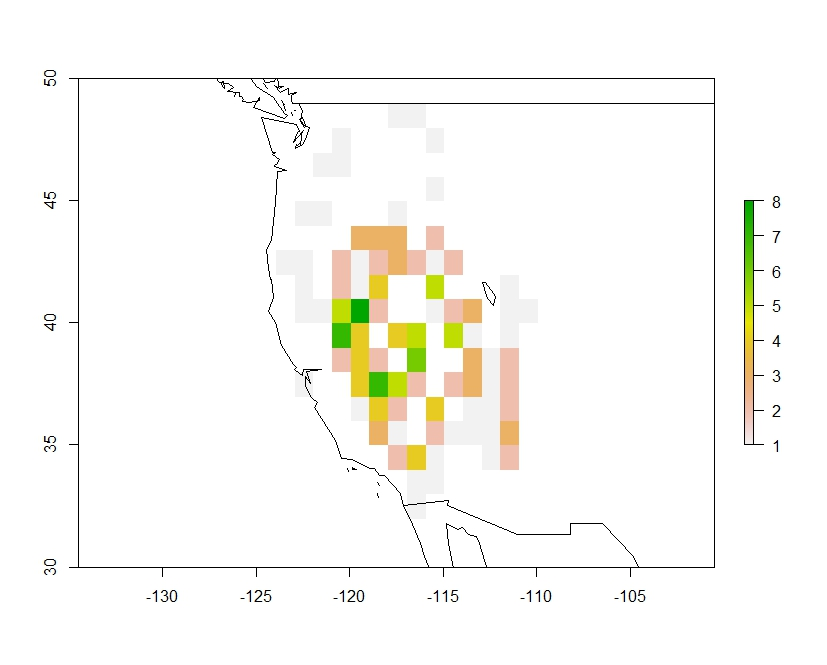
\includegraphics[width=0.7\textwidth]{figures/diversity_grid_textfile.jpeg}\\
\end{center}

Alternatively to using a input text file, you can also use the DiversityGrid() function on an object of the class "spgeoOUT" produced by the SpGeoCodH() function. In this case you can easily add the input points and/or your polygons to the plot.

\texttt{inp\_ivesia  \textless- ReadPoints(``example\_data\textbackslash \textbackslash ivesia\_coordinates.txt'', ``example\_data\textbackslash \textbackslash ivesia\_polygons.txt'')}\\
\texttt{outp\_ivesia \textless- SpGeoCodH(inp\_ivesia)}\\
\texttt{ivesia\_div \textless- DiversityGrid(outp\_ivesia, xlim = c(-130,-105), ylim = c(30,50))}\\
\texttt{MapGrid(ivesia\_div)}\\
\texttt{points(outp\_ivesia\$species\_coordinates\_in\$XCOOR, outp\_ivesia\$species\_coordinates\_in\$YCOOR)}\\
\texttt{plot(outp\_ivesia\$polygons, add = T, border =``grey50'')}

\begin{center}
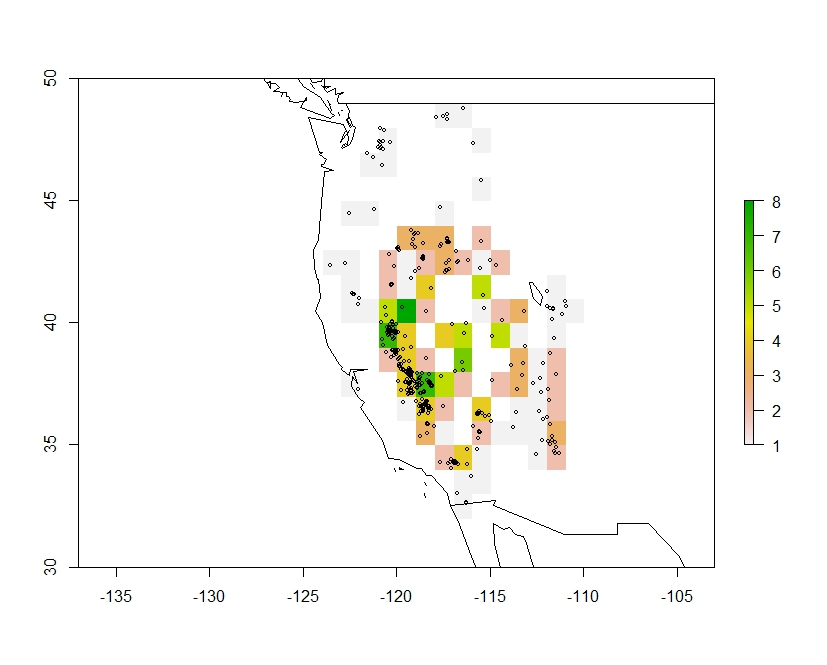
\includegraphics[width=0.7\textwidth]{figures/diversity_grid_spgeoout.jpeg}\\
\end{center}

If you want to represent the number of collection points in a grid you can use the AbundanceGrid() function similar to the DiversityGrid() function shown above.

\texttt{ivesia\_abu \textless- AbundanceGrid(outp\_ivesia, xlim = c(-130,-105), ylim = c(30,50))}\\
\texttt{MapGrid(ivesia\_abu)}\\
\texttt{points(outp\_ivesia\$species\_coordinates\_in\$XCOOR, outp\_ivesia\$species\_coordinates\_in\$YCOOR)}\\

\begin{center}
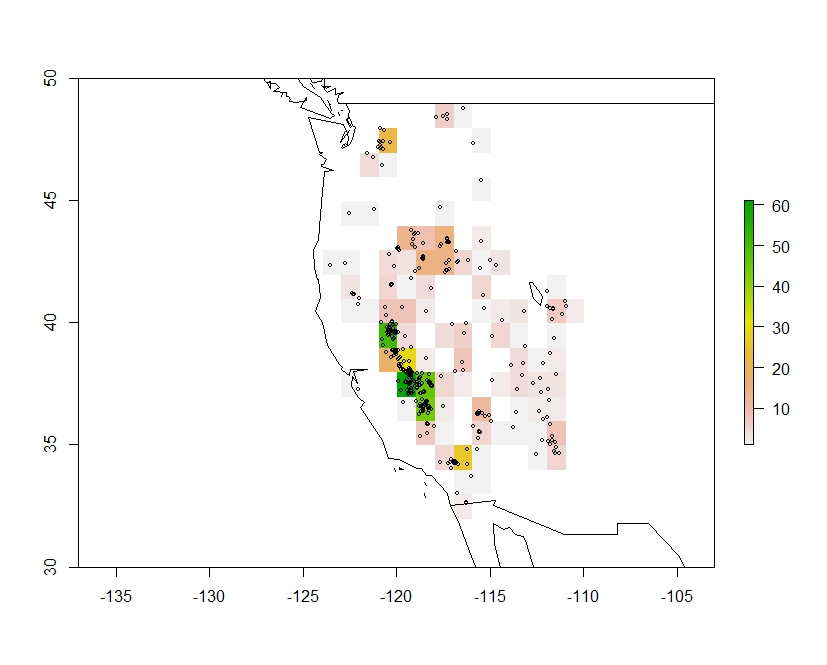
\includegraphics[width=0.7\textwidth]{figures/abundance_grid.jpeg}\\
\end{center}

\chapter{Function description} \label{functions}
\textbf{AbundanceGrid(x, xlim, ylim)}.\\
\textit{Input:} x = character string indicating the input file (same format as for SpeciesGeoCoder) or an object of the class "spgeoOUT"; xlim = vector indicating the minimum and maximum X coordinates (longitude, e.g. c(-10,10)); ylim = vector indicating the minimum and maximum Y coordinates (latitude, e.g. c(-10,10)).\\
\textit{Function:} creates a 1 degree grid and uses SpGeoCodH() to create a raster of the number of input points number per gridcell.\\
\textit{Output:} an raster object.\\
\\
\textbf{BarChartPoly(x, plotout, \dots)}\\
\textit{Input:} x = a object of class spgeoOUT; plotout = logical indicating if the function will be viewed in the R graphics device or passed to another output function, default is false.\\
\textit{Function:} this function gives out one bar chart per input polygon showing the number of occurrences for each species in this polygon.\\
\textit{Output:} a series of bar charts.\\
\\
\textbf{BarChartSpec(x, plotout,  \dots)}\\
\textit{Input:} x = a object of class spgeoOUT, plotout = logical (T/F).\\
\textit{Function:} this function gives out one bar chart per input species (or identifier) showing the number of occurrences in each polygon. plotout indicates if the function will be viewed in the R graphics device or passed to another output function, default = FALSE.\\
\textit{Output}: a series of bar charts.\\
\\
\textbf{CoExClass(x)}\\
\textit{Input:} x = class spgeoOUT.\\
\textit{Function:} this applies CoExClassH() to an object of class spgeoOUT, to add a species coexistence matrix to the object. This considers only species classified to polygons!\\
\textit{Output:} additional slot of the spgeoOUT object containing the coexistence matrix.\\
\\
\textbf{CoExClassH(x)}\\
\textit{Input:} x = data.frame of species occurrence numbers per polygon; ncol = number of polygons, nrow = number of species.\\
\textit{Function:} calculates a coexistence matrix of species. The number indicates the percentage of the species in the row co-occurring with the species in the column species in the row. This is the percentage of species classified to polygons!\\
\textit{Output:} data.frame, ncol= number of species + 1, nrow = number of species. The numbers indicate the percentage of the species in the row co-occurring with the species in the column.\\
\\
\textbf{ConvertPoly(x)}\\
\textit{Input:} a character vector indicating the path to a .txt file with polygon information exported from QGIS.\\
\textit{Function:} This function re-formats the dataframe to be suitable as input for the SpeciesGeoCoder() function.\\
\textit{Output:} a data.frame that can be exported for used as polygon input file for the SpeciesGeocoder() function.\\
\\
\textbf{Cord2Polygon(x)}\\
\textit{Input:} x = a tab delimited text file in the working directory OR a data.frame containing the Polygon information. Three columns: identifier, XCOOR, YCOOR.\\
\textit{Function:} creates spatial polygon objects out of point lists; Projection: latlon, wgs84.\\
\textit{Output:} SpatialPolygons object (=list of polygons).\\
\\
\textbf{CropPointCountry(x,y)}\\
\textit{Input:} x = a data.frame with coordinates of points of interest, 3 columns: identifier, XCOOR, YCOOR; y = a string or vector of strings with the countries of interest.\\
\textit{Function:} crops the point in x to the country borders of y, taken from the �wrld-simpl� data from the maptools package.\\
\textit{Output:} a data.frame, with points within the country borders.\\
\\
\textbf{CropPointPolygon(points, polygon, outside)}\\
\textit{Input:} points = data.frame, 3 columns: identifier XCOOR, YCOOR, polygon = polygon of interest as SpatialPolygons object, outside = logical value, T = points inside the polygons, F = points outside the polygons.\\
\textit{Function:} crops a data.frame with point coordinates to a polygon. Depending on outside it returns either a data.frame with the points lying inside or outside the polygon.\\
\textit{Output:} data.frame, with point coordinates.\\
\\
\textbf{DiversityGrid(x, xlim, ylim)}\\
\textit{Input:} x = character string indicating the input file (same formats as for SpeciesGeoCoder) or an object of the class "spgeoOUT", xlim = vector indicating the minimum and maximum X coordinates (longitude, e.g. c(-10,10)), ylim = vector indicating the minimum and maximum Y coordinates (latitude, e.g. c(-10,10)).\\
\textit{Function:} creates a 1 degree grid and uses spGeoCodH to create a raster of species number per cridcell.\\
\textit{Output:} an raster object.\\
\\
\textbf{*GetPythonIn(coordinates, polygon, sampletable, speciestable)}\\
\textit{Input:} coordinates =table of point coordinates, polygon = table of polygon coordinates, sampletable = results of species classification to polygons, speciestable = table of summary per species.\\
\textit{Function:} this is a helper function to pass the objects from the python code of the speciesgeocoder program.\\
\textit{Output:} object of class spgeoOUT.\\
\\
\textbf{HeatPlotCoEx(x, \dots)}\\
\textit{Input:} x = a object of class spgeoOUT OR a data.frame with ncol = identifier, number of species/identifiers; nrow = number of species/identifiers.\\
\textit{Function:} creates a heatplot from the coexistence matrix.\\
\textit{Output:} a single heat/level plot.\\
\\
\textbf{MapAll(x,polyg,moreborders)}\\
\textit{Input:} x = an object of class spgeoOUT, than polyg is not necessary, OR a matrix/data.frame of point coordinates 2 columns: XCOOR, YCOOR; polyg a SpatialPolygons object, with polygons of interest, moreborder = logical (T/F).\\
\textit{Function:} if method spgeoOUT than it maps all points and all polygons in the object. If method = matrix plots the points together with the polygons. The �moreborders� option adds borders of countries younger than 1990, default = F.\\
\textit{Output:} a plotted map.\\
\\
\textbf{MapDiversity(x, scale, leg = ``continous'', lim = ``polygons'', show.occ = F)}\\
\textit{Input:} x = a object of the class ``spgeoOUT''; scale the used for plotting must be one of c(``CUSTOM'',``ECOREGION'',``BIOME'',``REALM'') when used with polygons from an inputfile, scale = ``CUSTOM'', when used with polygons from the WWF ECOREGIONS, change accordingly; leg = either ``continous'' or ``discrete'', this controls the coloring scheme of the outputplot, default = ``continuous''; lim = either ``polygons'' or ``points'', controls if the plot limits should be derived from the input points or polygons; show.occ = T/F, controls if the occurrence points are shown in the plot.\\
\textit{Function:} this is wrapper function to colorcode diversity on the input polygons.\\
\textit{Output:} an R plot.\\
\\
\textbf{MapGrid(x)}\\
\textit{Input:} x = a raster object.\\
\textit{Function:} this is wrapper function to map a raster with country borders. Can be used with the results of DiversityGrid() and AbundanceGrid().\\
\textit{Output:} an R plot.\\
\\
\textbf{MapPerPoly(x, plotout)}\\
\textit{Input:} x = an object of class spgeoOUT; plotout = logical (T/F).\\
\textit{Function:} creates a series of maps, showing each polygon and its close environment, with all samples classified to this polygon. Species are color-coded. Plotout indicates if the function will be viewed in the R graphics device or passed to another output function, default = F. \\
\textit{Output:} a series of map plots.\\
\\
\textbf{MapPerSpecies(x, moreborders, plotout)}\\
\textit{Input:} x = an object of class spgeoOUT; moreboreders = logical (T/F); plotout = logical (T/F).\\
\textit{Function:} creates one map per species/identifier, showing all occurrence points related and all polygons. Plotout indicates if the function will be viewed in the R graphics device or passed to another output function, default = F. The �moreborders� option, add borders of countries younger than 1990, default = F.\\
\textit{Output}: a series of plotted maps.\\
\\
\textbf{MapUnclassified(x, moreborders, \dots)}\\
\textit{Input:} x = object of class spgeoOUT, moreboreders = logical, should additional borders be added?\\
\textit{Function:} creates a map of all input samples that could not be classified to one of the input polygons. The �moreborders� option, add borders of countries younger than 1990, default = F.\\
\textit{Output:} a plotted map.\\
\\
\textbf{NexusOut(x, verbose)}\\
\textit{Input:} x = an object of the class spgeoOUT, verbose = logical(T/F).\\
\textit{Function:} this function creates a table of the species classification to each area in nexus format for the further use in combination with phylogenetic trees. If verbose = T (default = F) the number of occurences per area are included in the file.\\
\textit{Output:} a .nex file in the working directory.\\
\\
\textbf{*OutBarChartPoly(x, \dots)}\\
\textit{Input:} x = object of class spgeoOUT.\\
\textit{Function:} produces a .pdf with a bar chart for each polygon showing the  number of occurrences for all input species in this specific polygon. This is a helper function producing the speciesgeocoder standard pdf from BarChartPoly().\\
\textit{Output:} �barchart\_per\_polygon.pdf� in the working directory.\\
\\
\textbf{*OutBarChartSpec(x, \dots)}\\
\textit{Input:} x = object of class spgeoOUT.\\
\textit{Function:} produces a .pdf with a bar chart for each species showing the occurrence in all input polygons. This is a helper function producing the speciesgeocoder standard .pdf from BarChartSpec().\\
\textit{Output:} �barchart\_per\_species.pdf� in the working directory.\\
\\
\textbf{*OutHeatCoEx(x, \dots)}\\
\textit{Input:} x = object of class spgeoOUT.\\
\textit{Function:} produces a .pdf showing a heat plot, representing the coexistence pattern between the input species. This is a helper function producing the speciesgeocoder standard pdf from HeatPlotCoEx().\\
\textit{Output:} �heatplot\_coexistence.pdf� in the working directory.\\
\\
\textbf{*OutMapAll(x, \dots)}\\
\textit{Input:} x = object of class spgeoOUT.\\
\textit{Function:} produces a .pdf showing a map of all points and a map of all points not classified to any polygon. This is a helper function producing the speciesgeocoder standard pdf from MapAll() and MapUnclassified().\\
\textit{Output:} �map\_samples\_overview.pdf� in the working directory.\\
\\
\textbf{*OutMapPerPoly(x, \dots)}\\
\textit{Input:} x = object of class spgeoOUT.\\
\textit{Function:} produces a .pdf showing a map of each polygon and its close environment with, all points that were classified to this polygon, color-coded by their identifier. This is a helper function producing the speciesgeocoder standard pdf from MapPerPoly().\\
\textit{Output:} �map\_samples\_per\_polygon.pdf� in the working directory.\\
\\
\textbf{*OutMapPerSpecies(x, \dots)}\\
\textit{Input:} x = object of class spgeoOUT.\\
\textit{Function:} produces a .pdf showing a map for each species with all polygons individuals of this species where classified to. This is a helper function producing the speciesgeocoder standard pdf from MapPerSpecies().\\
\textit{Output:} �map\_ per\_species.pdf� in the working directory.\\
\\
\textbf{*OutPlotSpPoly(x, \dots)}\\
\textit{Input:} x = object of class spgeoOUT.\\
\textit{Function:} produces a .pdf showing a bar chart of the species number per polygon. This is a helper function producing the speciesgeocoder standard .pdf from PlotSpPoly.\\
\textit{Output:} �number\_of\_species\_per\_polygon.pdf� in the working directory.\\
\\
\textbf{PipSamp(x)}\\
\textit{Input:} class spgeoIN.\\
\textit{Function:} calculates the homepolygon for each sample.\\
\textit{Output:} data frame; 2 columns: sample Id, containing polygon.\\
\\
\textbf{PlotOutSpGeo(x, \dots)}\\
\textit{Input:} x = an object of the class spgeoOUT.\\
\textit{Function:} This function calls all output functions, producing the standard package of output plots for speciesgeocoder.\\
\textit{Output:} .pdf files in the working directory.\\
\\
\textbf{PlotSpPoly(x,\dots)}\\
\textit{Input:} x = object of class spgeoOUT.\\
\textit{Function:} creates a bar chart on species numbers per polygon.\\
\textit{Output:} a bar chart.\\
\\
\textbf{PointInPolygon(x,y)}\\
\textit{Input:} x = data.frame with point coordinates; 3 columns: identifier, XCOOR, YCOOR ; y = data.frame with polygon points, 3 columns: identifierr, XCOOR, YCOOR. \\ 
\textit{Function:} performs a point in polygon test, and produces a table indicating the name of homepolygon of each sample as character string.\\
\textit{Output:} data.frame, 2 columns: identifier, homepolygon.\\
\\
\textbf{ReadPoints(x,y)}\\
\textit{Input:} Two text files in the working directory: x = coordinates of the points of interest, y = the coordinates of the polygons. 3 Columns: identifier, XCOOR, YCOOR.\\
\textit{Function:} creates an object of the class spgoeIN (= list of pointidentifiers, point coordinate, spatial polygons.\\
\textit{Output:} object of class spgeoIN.\\
\\
\textbf{SpeciesGeoCoder(x, y, coex, graphs)}\\
\textit{Input:} Two text files in the working directory: x = coordinates of the points of interest, y = the coordinates of the polygons. 3 Columns: identifier, XCOOR, YCOOR.\\
\textit{Function:} the main function of the package. This performs the whole species geocoder and produces the standard package of output files. Produces a number of standard output-tables containing: 1. classification of all samples to a polygon, 2. Summary of species (identifier) occurrence per polygon, 3. A table of samples that could not be classified to any of the input polygons, 4. a Nexus-file, including the species classification, 5. A coexistence matrix, showing to which percentage species to co-occurr in the input polygons, 5. A table giving species numbers per polygon. Furthermore produces a set of .pdf files in the output directory: 1. A barchart showing the number of species per polygon, 2. a barchart summarizing numbers of each species for each polygon, 3. A bar chart summarizing the occurrences in each polygon per species, 4. A map of all polygons with the points classified to them, colored for species (identifier), 5. a map of the occurrences of all species, A map showing all points used and all unclassified points in the geographic context, 6. A heat plot showing the co-occurrence patterns of all species in the polygons.\\
\textit{Output:} multiple tab-delimited tables and graphics in pdf format.\\
\\
\textbf{SpGeoCod(x, y)}\\
\textit{Input:} x = .txt file containing the information of species occurrence, 3 columns: identifier, XCOOR, YCOOR; y = points comprising the polygons, 3 columns: identifier, XCOOR, YCOOR.\\
\textit{Function:} this function combines ReadPoints() and SpGeoCodH() to produce an object of the class spgeoOUT from input text files.\\
\textit{Output:} object of class spgeoOUT.\\
\\
\textbf{SpGeoCodH(x)}\\
\textit{Input:} object of class spgeoIN.\\
\textit{Function:} this is one of the core functions. It uses an object of the class spgeoIN and performs appoint in polygon test classifying each species to a polygon, summarizes the information per species, summarizes the number of species per polygon, produces a table  showing the samples that could not be classified and calculates a coexistence matrix. These objects are then put together with the input information to an object of the class spgeoOUT.\\
\textit{Output:} spgeoOUT.\\
\\
\textbf{spPerPol(x)}\\
\textit{Input:} class spgeoIN.\\
\textit{Function:} combines PipSamp(), SpSumH and SpPerPolH;\\
\textit{Output:} a named vector with species number per polygon.\\
\\
\textbf{*spPerPolH(x)}\\
\textit{Input:} data.frame, ncol = number of polygons, nrow = number of species. This is a helper function, which takes input directly from SpSumH().\\
\textit{Function:} calculates the number of species per polygon.\\
\textit{Output:} a named vector, with species number per polygon.\\
\\
\textbf{spSum(x)}\\
\textit{Input:} x = object of class spgeoIN.\\
\textit{Function:} calculates a summary of the number of species occurrences per polygon.\\
\textit{Output:} a data.frame summarizing the occurrence number of species per polygon; ncol = number of polygons, nrow = number of species.\\
\\
\textbf{*spSumH(x)}\\
\textit{Input:} x = class spgeodataframe, this is a helper function to take output from pipSamp.\\
\textit{Function:} calculates a summary of species occurrences from a 2 column table: identifier, hompolygon.\\
\textit{Output:} A data.frame summarizing the occurrence number of species per polygon.\\
Uses output of pipSamp to give out a dataframe of number of species occurrences per polygon, ncol = number of polygons, nrow = number of species.\\
\\
\textbf{WriteTablesSpGeo(x, \dots)}\\
\textit{Input:} object of class spgeoOUT.\\
\textit{Function:} creates 5 output - tables as tab delimited text files in the working directory: 1. classification of all samples to a polygon, 2. Summary of species (identifier) occurrence per polygon, 3. A table of samples that could not be classified to any of the input polygons, 4. A coexistence matrix, showing to which percentage species to co-occur in the input polygons, 5. A table giving species numbers per polygon.\\
\textit{Output:} tab delimited .txt files in the working directory.\\
\\
\textbf{WWFconvert(x)}\\
\textit{Input:} x = SpatialPolygonsDataframe object of the biomes and ecoregions of the WWF or any subset of it. Available from http://maps.tnc.org/gis\\data.html, and loaded to R with readShapeSpatial() from the raster package.\\
\textit{Function:} converts the polygons in the object to a list of points.\\
\textit{Output:} data.frame, 3 columns: identifier, XCOOR, YCOOR.\\
\\
\textbf{WWFload()}
\textit{Input:} no input arguments needed.\\
\textit{Function:} dowloads the WWF terrestrial ecoregions layer \citep{olson2001} from the WWF hompage and unzips the files in the working directory.\\
\textit{Output:} the shape is loaded and assigned to the object traget of the function, e.g. wwf \textless- WWFload().\\
\\
\textbf{WWFnam(x)}\\
\textit{Input:} x = a SpatialPolygonsDataFrame of the biomes and ecoregions of the WWF or any subset of it. Available from http://maps.tnc.org/gis\\data.html, and loaded to R with readShapeSpatial() from the raster package.\\
\textit{Function:} shows all available subset categories for the of the dataset for WWFpick() and WWFpoly2point().\\
\textit{Output:} A list of strings.\\
\\
\textbf{WWFpick(x, name, scale)}\\
\textit{Input:} x = a SpatialpolygonsDataFrame of the biomes and ecoregions of the WWF or any subset of it. Available from http://maps.tnc.org/gis\\data.html, and loaded to R with readShapeSpatial() from the raster package; name = name of the realm, biome or ecoregion of interest, scale = character string indicating the scale of interest (one of: �REALM�, �BIOME�, �ECOREGION�).\\
\textit{Function:} creates a subset of the WWF ecoregion Polygons.\\
\textit{Output:} class SpatialPolygonsDataFrame.\\
\\
\textbf{WWFpoly2point(x, name, scale)}\\
\textit{Input:} x = a SpatialPolygonsDataFrame of the biomes and ecoregions of the WWF or any subset of it. Available from http://maps.tnc.org/gis\\data.html, and loaded to R with readShapeSpatial() from the raster package; name = name of the realm, biome or ecoregion of interest, scale = character string indicating the scale of interest (one of: �REALM�, �BIOME�, �ECOREGION�).\\
\textit{Function:} combines WWFpick() and WWFconvert(). Produces a list of points defining the realm, biome or ecoregion defined in the input.\\
\textit{Output:} data.frame, 3 columns, identifier, XCOOR, YCOOR.\\

\chapter{Benchmarking} \label{benchmark}
SpeciesgeocodeR was explicitly designed for the analysis of large datasets. Most analyses should run within minutes. However, very large datasets might need longer. To give you an idea of the expected computation time for you dataset using the SpeciesGeoCoder() function this chapter shows some result of benchmarking tests. The computational time is show against the number of data-points in your dataset. The figures also show the impact of polygon number and polygon complexity, as well as the additional time needed when the graphical output is switched on. When using very large datasets, please note that R reads all information into the memory, and that there is a limit of 2 GB that can be allocated to a single vector.
\newpage

\centering
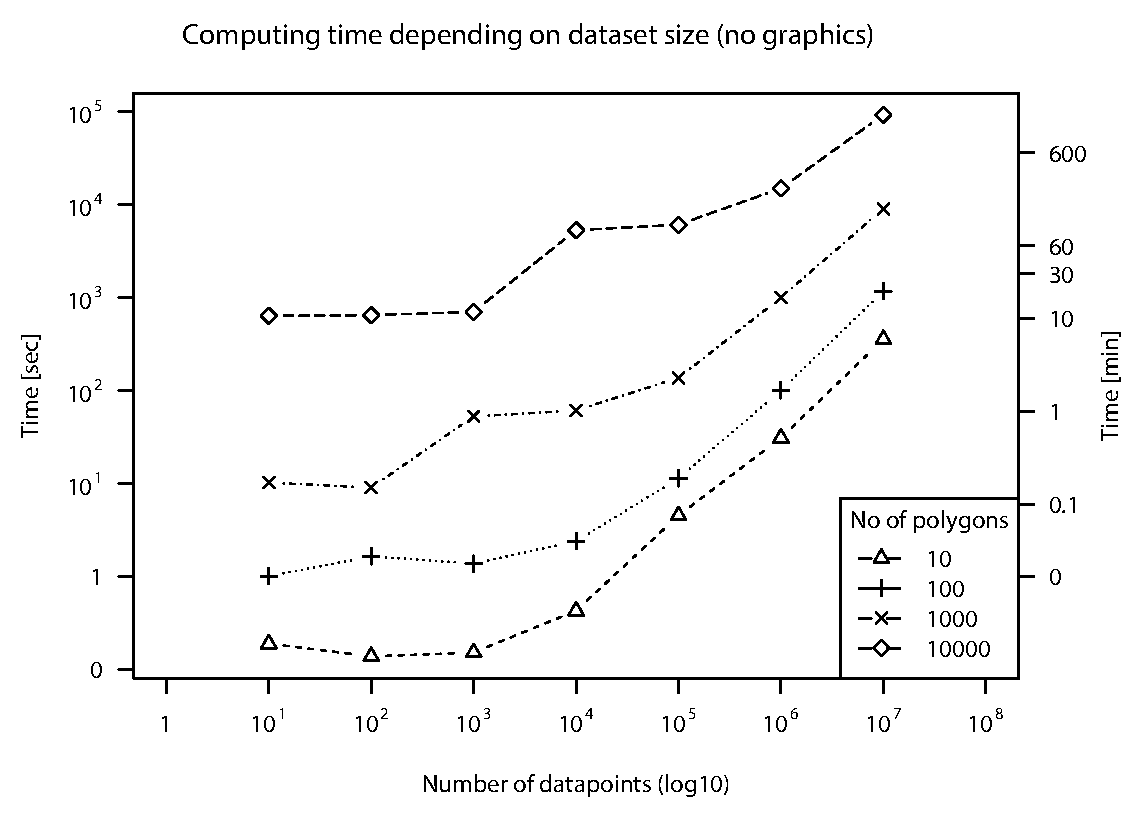
\includegraphics[width=0.9\textwidth]{figures/bm_no_graphics.eps}\\
\vspace{2cm}
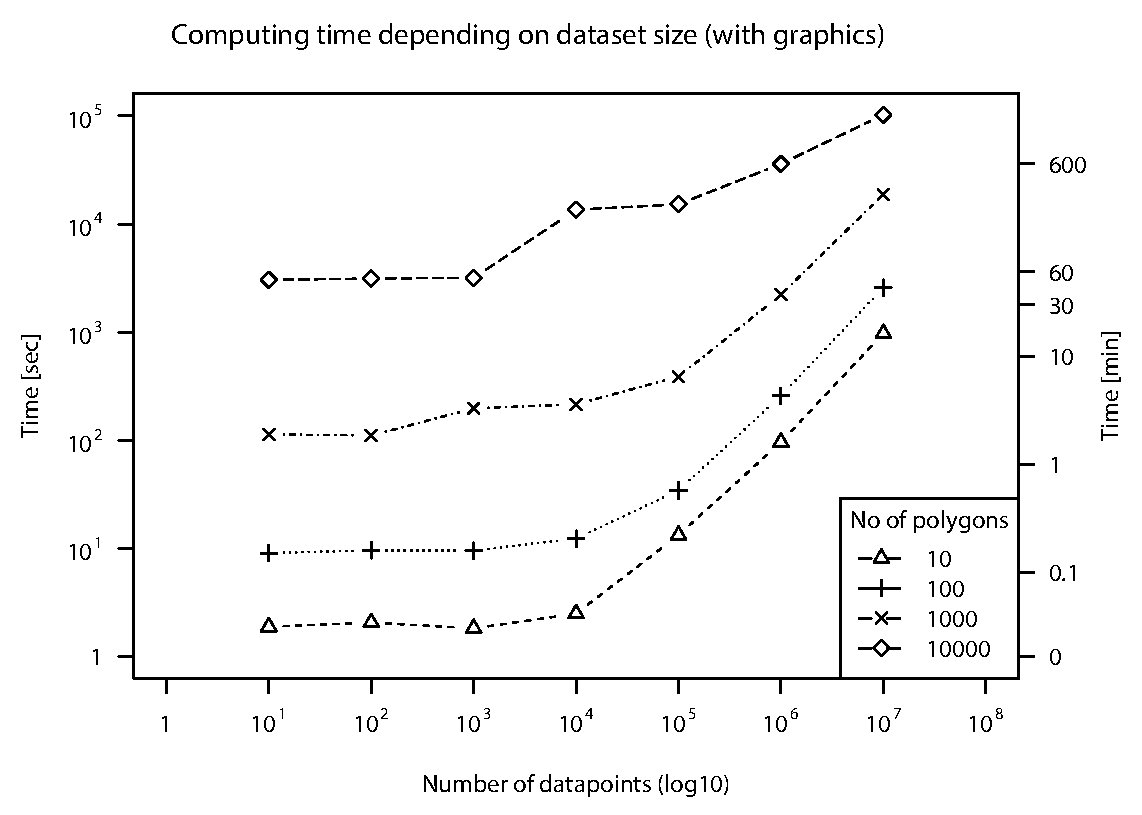
\includegraphics[width=0.9\textwidth]{figures/bm_graphics.eps}


\bibliography{literature}{}


\end{document}